%%%%%%%%%%%%%%%%%%%%%%%%%%%%%%%%%%%%%%%%%%%%%%%%%%%%%%%%%%%%%%%%%%%%%%%%%%%%%%%%
%%%%%%%%%%%%%%%%%%%%%%%%%%%%%%%%%%%%%%%%%%%%%%%%%%%%%%%%%%%%%%%%%%%%%%%%%%%%%%%%
%%% Template for AIMS Rwanda Assignments         %%%              %%%
%%% Author:   AIMS Rwanda tutors                             %%%   ###        %%%
%%% Email: tutors2017-18@aims.ac.rw                               %%%   ###        %%%
%%% Copyright: This template was designed to be used for    %%% #######      %%%
%%% the assignments at AIMS Rwanda during the academic year %%%   ###        %%%
%%% 2017-2018.                                              %%%   #########  %%%
%%% You are free to alter any part of this document for     %%%   ###   ###  %%%
%%% yourself and for distribution.                          %%%   ###   ###  %%%
%%%                                                         %%%              %%%
%%%%%%%%%%%%%%%%%%%%%%%%%%%%%%%%%%%%%%%%%%%%%%%%%%%%%%%%%%%%%%%%%%%%%%%%%%%%%%%%
%%%%%%%%%%%%%%%%%%%%%%%%%%%%%%%%%%%%%%%%%%%%%%%%%%%%%%%%%%%%%%%%%%%%%%%%%%%%%%%%


%%%%%% Ensure that you do not write the questions before each of the solutions because it is not necessary. %%%%%% 

\documentclass[12pt,a4paper]{article}

%%%%%%%%%%%%%%%%%%%%%%%%% packages %%%%%%%%%%%%%%%%%%%%%%%%
\usepackage{amsmath}
\usepackage{amssymb}
\usepackage{amsthm}
\usepackage{amsfonts}
\usepackage{graphicx}
\usepackage[all]{xy}
\usepackage{tikz}
\usepackage{verbatim}
\usepackage[left=2cm,right=2cm,top=3cm,bottom=2.5cm]{geometry}
\usepackage{hyperref}
\usepackage{caption}
\usepackage{subcaption}
\usepackage{psfrag}

%%%%%%%%%%%%%%%%%%%%% students data %%%%%%%%%%%%%%%%%%%%%%%%
\newcommand{\student}{Akor Stanley}
\newcommand{\course}{DA }
\newcommand{\assignment}{2}

%%%%%%%%%%%%%%%%%%% using theorem style %%%%%%%%%%%%%%%%%%%%
\newtheorem{thm}{Theorem}
\newtheorem{lem}[thm]{Lemma}
\newtheorem{defn}[thm]{Definition}
\newtheorem{exa}[thm]{Example}
\newtheorem{rem}[thm]{Remark}
\newtheorem{coro}[thm]{Corollary}
\newtheorem{quest}{Question}[section]

%%%%%%%%%%%%%%  Shortcut for usual set of numbers  %%%%%%%%%%%

\newcommand{\N}{\mathbb{N}}
\newcommand{\Z}{\mathbb{Z}}
\newcommand{\Q}{\mathbb{Q}}
\newcommand{\R}{\mathbb{R}}
\newcommand{\C}{\mathbb{C}}
%%%%%%%%%%%%%%%%%%%%%%%%%%%%%%%%%%%%%%%%%%%%%%%%%%%%%%%555
\begin{document}
%%%%%%%%%%%%%%%%%%%%%%% title page %%%%%%%%%%%%%%%%%%%%%%%%%%
\thispagestyle{empty}
\begin{center}
\textbf{AFRICAN INSTITUTE FOR MATHEMATICAL SCIENCES \\[0.5cm]
(AIMS RWANDA, KIGALI)}
\vspace{1.0cm}
\end{center}
%%%%%%%%%%%%%%%%%%%%% assignment information %%%%%%%%%%%%%%%%
\noindent
\rule{17cm}{0.2cm}\\[0.3cm]
Name: \student \hfill Assignment Number: \assignment\\[0.1cm]
Course: \course \hfill Date: \today\\
\rule{17cm}{0.05cm}
\vspace{1.0cm}
\section*{Question 1}
From Bayes theorem;
\begin{itemize}
	\item [(a)]
\begin{align}
f_{X|Y}=\frac{f_{Y|X}(Y|X)f_{X}(X)}{f_{Y}(Y)}\\
f_{X|Y} \propto f_{Y|X}(Y|X)f_{X}(X) \label{1}
\end{align}
But;
\begin{align*}
f_{Y|X}& \propto \exp\left[-\frac{1}{2}\sum_{i=1}^{N}\left(\frac{y_{i}-x}{\tau} \right)^{2}\right]\\
f_{Y|X}&\propto \exp\left[-\frac{1}{2}\left(\sum_{i=1}^{N}\frac{y_{i}^{2}-2y_{i}x}{\tau^{2}}+\frac{Nx^{2}}{\tau^{2}}\right)\right]
\end{align*}
Similarly,
\begin{align*}
f_{X}(X)=\exp \left[-\frac{1}{2}\left(\frac{x-\mu}{\sigma}\right)^{2}\right]
\end{align*}
Applying equation\ref{1}, we shall have;
\begin{align*}
f_{X|Y} &\propto \exp\left[-\frac{1}{2}\left(\sum_{i=1}^{N}\frac{y_{i}^{2}-2y_{i}x}{\tau^{2}}+\frac{Nx^{2}}{\tau^{2}}\right)\right]\centerdot \exp \left[-\frac{1}{2}\left(\frac{x-\mu}{\sigma}\right)^{2}\right]\\
f_{X|Y}&\propto\left[-\frac{1}{2}\left(\sum_{i=1}^{N}\frac{y_{i}^{2}}{\tau^{2}}+\frac{\mu^{2}}{\sigma^{2}}-\frac{2y_{i}x}{\tau^{2}}+\frac{2\mu x}{\sigma^{2}}+\frac{x^{2}}{\sigma^{2}}+\frac{Nx^{2}}{\tau^{2}}\right)\right]\\
f_{X|Y}&\propto\left[-\frac{1}{2}\left(\left(\sum_{i=1}^{N}\frac{y_{i}^{2}}{\tau^{2}}+\frac{\mu^{2}}{\sigma^{2}}\right)-2x\left(\sum_{i=1}^{N}\frac{y_{i}}{\tau^{2}}+\frac{\mu}{\sigma^{2}}\right)+x^{2}\left(\frac{N}{\tau^{2}}+\frac{1}{\sigma^{2}}\right)\right)\right]\\
\end{align*}
\begin{align}
f_{X|Y}&\propto\exp\left[-\frac{1}{2}\left(\sum_{i=1}^{N}\frac{y_{i}^{2}}{\tau^{2}}+\frac{\mu^{2}}{\sigma^{2}}\right)\right]\exp\left[-\frac{1}{2}\left(-2x\left(\sum_{i=1}^{N}\frac{y_{i}}{\tau^{2}}+\frac{\mu}{\sigma^{2}}\right)+x^{2}\left(\frac{N}{\tau^{2}}+\frac{1}{\sigma^{2}}\right)\right)\right] \label{6}
\end{align}
We shall ignore the first term of our exponent in equation\ref{6} because it is independent of $x$. Therefore;
\begin{align}
f_{X|Y}&\propto\left[-\frac{1}{2}\left(-2x\left(\sum_{i=1}^{N}\frac{y_{i}}{\tau^{2}}+\frac{\mu}{\sigma^{2}}\right)+x^{2}\left(\frac{N}{\tau^{2}}+\frac{1}{\sigma^{2}}\right)\right)\right] \label{4}
\end{align}
\item [(b)]
In order to use the completing the squares method, we make some simplification to equation\ref{4}. So let;
\begin{align*}
Q&=\left(\frac{N}{\tau^{2}}+\frac{1}{\sigma^{2}}\right)\\
R&=\left(\sum_{i=1}^{N}\frac{y_{i}}{\tau^{2}}+\frac{\mu}{\sigma^{2}}\right)
\end{align*}
Equation\ref{4} now becomes;
\begin{align*}
f_{X|Y}&\propto \exp\left[-\frac{1}{2}\left(Qx^{2}-2Rx\right)\right]\\
f_{X|Y}&\propto \exp \left[-\frac{Q}{2}\left(x^{2}-\frac{2Rx}{Q}\right)\right]
\end{align*}
Now by applying completing the squares to the simplified distribution, we shall have;
\begin{align*}
f_{X|Y}&\propto \exp\left[-\frac{Q}{2}\left(\left(x-\frac{R}{Q}\right)^{2}-\left(\frac{R}{Q}\right)^{2}\right)\right]\\
f_{X|Y}&\propto\exp\left[-\frac{Q}{2}\left(x-\frac{R}{Q}\right)^{2}\right]\exp\left[\frac{Q}{2}\left(\frac{R}{Q}\right)^{2}\right]
\end{align*}
Since the second exponential is independent of $x$, it is assumed to be a constant in this situation, Hence;
\begin{align*}
f_{X|Y}&\propto \exp\left[-\frac{Q}{2}\left(x-\frac{R}{Q}\right)^{2}\right]\\
&\propto \exp\left[\frac{-\frac{1}{2}\left(x-\frac{R}{Q}\right)^{2}}{\frac{1}{Q}}\right]
\end{align*}
$f_{X|Y}$, is a gaussian distribution with mean $\frac{R}{Q}$, therefore;
\begin{align*}
\mu^{*}&=\frac{R}{Q}=\frac{\left(\sum_{i=1}^{N}\frac{y_{i}}{\tau^{2}}+\frac{\mu}{\sigma^{2}}\right)}{\left(\frac{N}{\tau^{2}}+\frac{1}{\sigma^{2}}\right)}\\
&=\left(\frac{N}{\tau^{2}}+\frac{1}{\sigma^{2}}\right)^{-1}\left(\sum_{i=1}^{N}\frac{y_{i}}{\tau^{2}}+\frac{\mu}{\sigma^{2}}\right)
\end{align*}
The variance is given by;
\begin{align*}
Var(X|Y)&=\frac{1}{Q}\\
&=\left(\frac{N}{\tau^{2}}+\frac{1}{\sigma^{2}}\right)^{-1}
\end{align*}
\item [(c)]
We have;

From our expression of the posterior mean;
\begin{align*}
\mu^{*}=\frac{\left(\sum_{i=1}^{N}\frac{y_{i}}{\tau^{2}}+\frac{\mu}{\sigma^{2}}\right)}{\left(\frac{N}{\tau^{2}}+\frac{1}{\sigma^{2}}\right)}
\end{align*}
We shall simplify expressions in $\mu^{*}$ by making the following computation;
\begin{align*}
\sum_{i=1}^{N}\frac{y_{i}}{\tau^{2}}=\sum_{i=1}^{N}\frac{N}{N}\frac{y_{i}}{\tau^{2}}=\frac{N}{\tau^{2}}\sum_{i=1}^{N}\frac{y_{i}}{N}=\frac{N}{\tau^{2}}\bar{y}
\end{align*}
Therefore;
\begin{align*}
\mu^{*}&=\frac{\frac{N}{\tau^{2}}\bar{y}+\frac{\mu}{\sigma^{2}} }{\frac{N}{\tau^{2}}+\frac{1}{\sigma^{2}}}\\
&=\frac{N\bar{y}\sigma^{2}+ \mu\tau^{2}}{N\sigma^{2}+ \tau^{2}}\\
&=\frac{N\bar{y}\sigma^{2}+ \mu\tau^{2}+\mu(N\sigma^{2}+\tau^{2})-\mu(N\sigma^{2}+\tau^{2})}{N\sigma^{2}+ \tau^{2}}\\
&=\mu + \frac{N\bar{y}\sigma^{2}+ \mu\tau^{2}-\mu(N\sigma^{2}+\tau^{2})}{N\sigma^{2}+ \tau^{2}}\\
&=\mu +\frac{N\sigma^{2}(\bar{y}-\mu)}{N\sigma^{2}+ \tau^{2}}\\
\mu^{*}&=\mu +k(\bar{y}-\mu)
\end{align*}
\item [(cii)]
Given; $$\mu^{*}=\mu +k(\bar{y}-\mu)$$
By expansion, we obtain;
\begin{align*}
\mu^{*}&=\mu + \frac{N\sigma^{2}}{N\sigma^{2}+ \tau^{2}}\centerdot \bar{y}- \frac{N\sigma^{2}}{N\sigma^{2}+ \tau^{2}}\centerdot \mu\\
&=\left(1-\frac{N\sigma^{2}}{N\sigma^{2}+ \tau^{2}}\right)\mu + \frac{N\sigma^{2}}{N\sigma^{2}+ \tau^{2}}\centerdot \bar{y}\\
&=\frac{\tau^{2} }{N\sigma^{2}+ \tau^{2}} \centerdot \mu+ \frac{N\sigma^{2}}{N\sigma^{2}+ \tau^{2}}\centerdot \bar{y}
\end{align*}
\item [(d)] The posterior mean is given by;
\begin{align}
\mu^{*}&=\mu +\frac{N\sigma^{2}(\bar{y}-\mu)}{N\sigma^{2}+ \tau^{2}} \label{9}
\end{align}
\begin{itemize}
	\item [d(i)] As $\tau^{2} \rightarrow \infty$, then the equation of the  posterior mean $\mu^{*}$ becomes;
	$$\mu^{*}\approx\mu$$
	That is, the posterior mean becomes equivalent to the prior mean.
	\item[d(ii)] As $N\rightarrow \infty$, and the uncertainty of $\tau$ is fixed, then the equation of the posterior mean $\mu^{*}$ becomes;
	\begin{align*}
	\mu^{*}\approx \bar{y}
	\end{align*}
	That is, the posterior mean becomes equivalent to the mean of all the observations.
\end{itemize}
\item[(e)]
We have seen that the Var$(X|y)$ is given by
\begin{align*}
Var(X|y)&=\left(\frac{N}{\tau^{2}}+\frac{1}{\sigma^{2}}\right)^{-1}\\
&=\frac{\tau^{2}\sigma^{2}}{N\sigma^{2}+\tau^{2}}\\
&=\frac{\tau^{2}}{N\sigma^{2}+\tau^{2}}\sigma^{2}
\end{align*}
We have been given the expression that $k=\frac{N\sigma^{2}}{N\sigma^{2}+\tau^{2}}$, thus;
\begin{align}
(1-k)\sigma^{2}&=\left(1-\frac{N\sigma^{2}}{N\sigma^{2}+\tau^{2}}\right)\sigma^{2}\\
&=\left(\frac{\tau^{2}}{N\sigma^{2}+\tau^{2}}\right)\sigma^{2} \label{8}
\end{align}
Hence, we have shown that Var$(X|Y)=(1-k)\sigma^{2}$\\
From equation\ref{8}, as $\tau^{2} \rightarrow \infty$, then $Var(X|Y)=\sigma^{2}$. However, as $N\rightarrow \infty$, $Var(X|Y)=0$
\end{itemize}
\section*{Question 2}
\begin{itemize}
	\item [(a)] The parametres in the kalman filter formular are;
	\begin{align*}
	M_{t}=0.7\textbf{I}_{1}\\
	H_{t}=1\\
	\Sigma_{t}=1\\
	R_{t}=0.1\\
	Q_{t}=0.5
	\end{align*}
	\item [(b)] The dimensions are
	\begin{align*}
	\textbf{K}_{t}\in \R\\
	\boldsymbol{\mu}_{t|t-1}\in \R\\
	\boldsymbol{\Sigma}_{t|t-1}\in \R\\
	\boldsymbol{\mu}_{t|t}\in \R\\
	\boldsymbol{\Sigma}_{t|t}\in \R
	\end{align*}
	\newpage
	\item [(c)]Figure\ref{f1} shows the simulation of our process model for $t=1,.......,100$	
	\begin{figure}[h!]
		\centering
		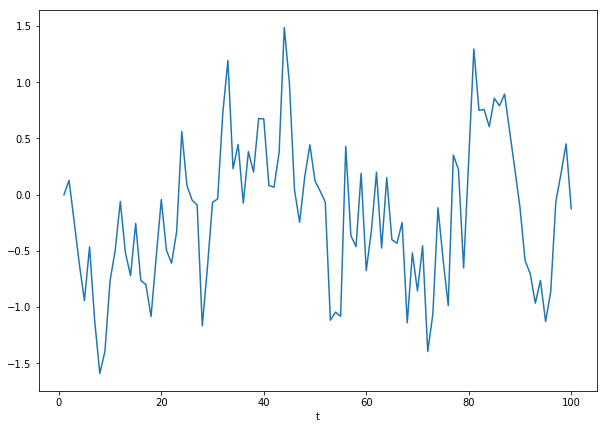
\includegraphics[scale=0.5]{a.png}
		\caption{Process Model Simulation} \label{f1}
	\end{figure}
	
	\item [(d)].\\	
	Figure\ref{fig2}, shows a plot of the truth $x_{t}$ and data $y_{t}$ for $t=1,.......,100$, excluding points $40,..,43$ and $80,...,83$
	\begin{figure}[h!]
		\centering
		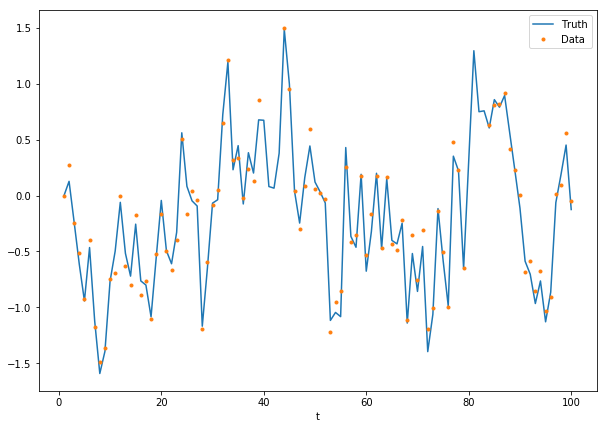
\includegraphics[scale=0.5]{b.png}
		\caption{Simulation of the Process Model and Data} \label{fig2}
	\end{figure}
\newpage
	\item [(e)]Figure\ref{fig3} below shows the plot of the kalman estimate, process model, and the data. Carefully inspecting the plot, one can observe that the kalman estimates are often lying between the noise observations and the truth states. However from $t=40,..,43$ and $t=80,..,83$, we observe that the kalman estimates are far away from the truth states, this is because data is not available within those points
	\begin{figure}[h!]
		\centering
		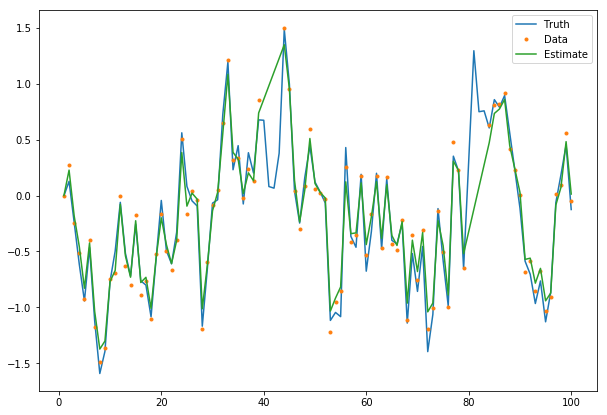
\includegraphics[scale=0.5]{c.png} 
		\caption{Simulation of the Process Model, Data and Kalman Estimate} \label{fig3}
	\end{figure}
\end{itemize}
\end{document}